
%%%%%%%%%%%%%%%%%%%%%%%%%%%%%%%%%%%%%%%%%%%%%%%%%%%%%%%%%%%%%%%%%%%%%%%%%
%           Capítulo 2: MARCO TEÓRICO - REVISIÓN DE LITERATURA
%%%%%%%%%%%%%%%%%%%%%%%%%%%%%%%%%%%%%%%%%%%%%%%%%%%%%%%%%%%%%%%%%%%%%%%%%
\chapter{Antecedentes}

En este capítulo se presentan los principales antecedentes de la aeronave de ala-integrada.
Sus primeros diseños, características, ventajas y principales retos. Finalmente, se da una breve descripción de los sistemas de control de vuelo de los principales modelos a escala de Boeing y Airbus. 


%%%%%%%%%%%%%%%%%%%%%%%%%%%%%%%%%%%%%%%%%%%%%%%%%%%%%%%%%%%%%%%%%%%
\section{Aeronave de Ala-Integrada (BWB)}

La aviación es un punto de interés global, dónde uno de los aspectos que han ocupado la atención de las principales empresas aeroespaciales como Boeing y Airbus, es su impacto ambiental. Entre las principales fuentes contaminantes tenemos al ruido, las emisiones contaminantes de dióxido de carbono ($CO_2$) y óxidos de nitrógeno ($NOx$). 
%
En la Figura \ref{fig: emisiones de la aviación comercial} podemos observar el contraste de las emisiones de $CO2$ globales respecto a las emitidas por la aviación comercial en una línea del tiempo hasta 2015. Las emisiones de la aviación comercial contribuyen con el  $2\%$ de las emisiones globales.
%
\begin{figure}[h]
\centering
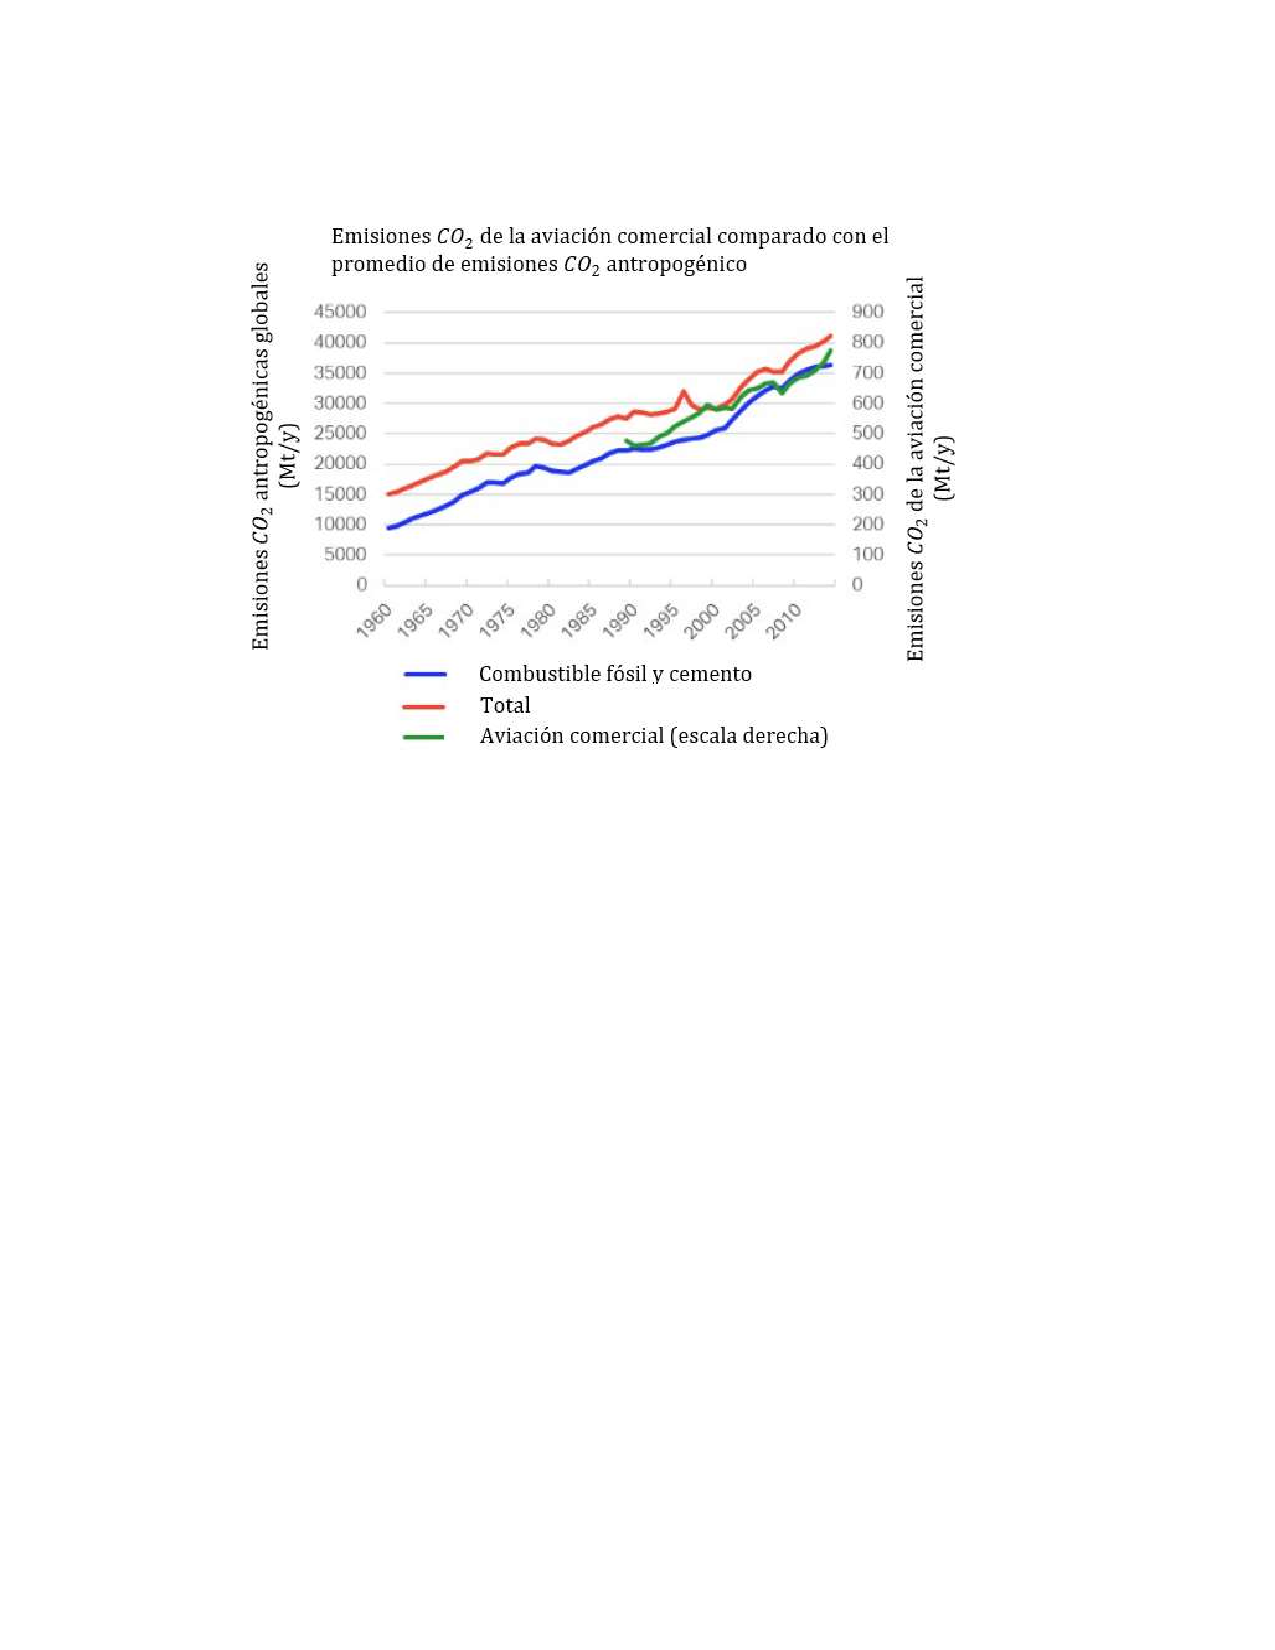
\includegraphics[scale=0.75]{Capitulo3/figs/emsisiones CO2 global y aviacion_cropped.pdf}
\caption{Emisiones $CO_2$ antropogénicas globales y de la aviación comercial  \cite{IATA2020}}
\label{fig: emisiones de la aviación comercial}
\end{figure}
%
Asimismo, en base a los informes anuales de Boeing y Airbus \cite{OneAir}, se observa que en los últimos 15 años el número de pasajeros que utilizan un avión se ha triplicado. 
%
Sólo en 2019, 4.5 millones de personas viajaron en una de las 1300 líneas aéreas que concentran un total de 26,000 aeronaves alrededor del mundo, y las cuales hicieron 40 millones de vuelos sólo en ese año.
%
Adicionalmente, de acuerdo a un estudio de Airbus y la Organización de Aviación Civil Internacional (\textit{ICAO}) se presenta un pronostico de como entre 2021 a 2041 variarán los pasajeros-kilometro (\textit{RPK, en inglés}), ver Figura \ref{pronostico RPK 2021-2041}.
%
\begin{figure}[h]
\centering
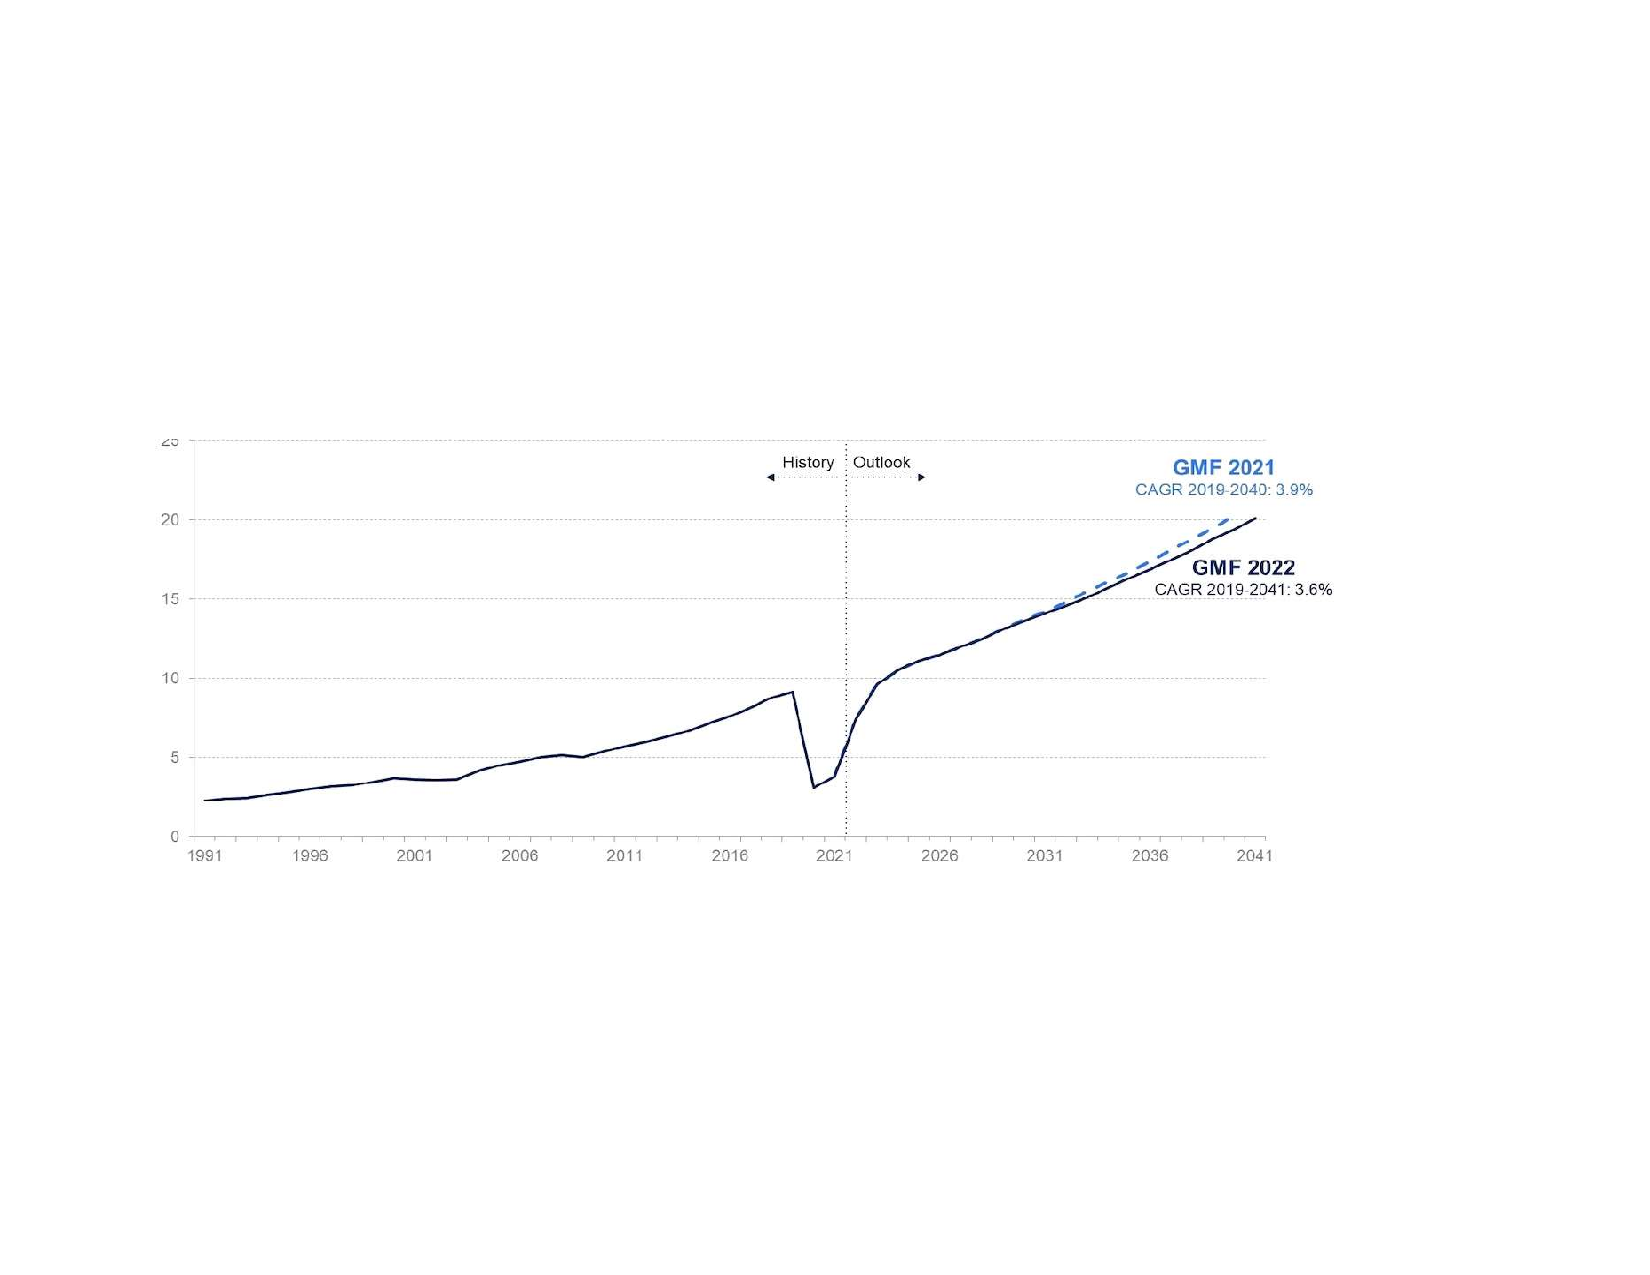
\includegraphics[scale=0.6]{Capitulo3/figs/pronostico AirbusICAO 2041_cropped.pdf}
\caption{Pronóstico en trillones de ingresos por pasajero-kilometro 2021-2041\cite{OneAir}}
\label{pronostico RPK 2021-2041}
\end{figure}
%

Como acciones para corregir este problema, desde 2009 la industria entera de la aviación (aerolíneas, compañías de manufactura aeroespaciales, aeropuertos, proveedores de servicios de navegación y negocios de aviación) estableció los objetivos climáticos de alto-nivel:
\begin{itemize}
    \item Mejorar la eficiencia del  combustible en $1.5 \%$ por año entre el periodo de 2009-2020. 
    \item Alcanzar un crecimiento neutral neto de emisiones de carbono a partir del 2020.
    \item Reducir las emisiones globales netas de carbono en un $50 \%$ por ciento para el año 2050 respecto al año 2005. 
\end{itemize}
%
%
Es importante mencionar que la reducción de emisiones contaminantes es un reto que requiere la combinación de todas las posibles contribuciones de las partes interesadas y en todos los pilares de la estrategia de la Asociación Internacional del Transporte Aéreo (IATA, en inglés). 
%
En este sentido, se considera que desde 2035 en adelante, podrían hacerse realidad tecnologías radicales e innovadoras con una alta eficiencia en rendimiento y combustible como son nuevas configuraciones de aeronaves sobre la convencional actual TAW, y nuevas formas de fuentes de energía para el sistema de propulsión; como baterías eléctricas, celdas de hidrógeno y propuestas híbridas. 
%
En la Figura \ref{tecnologías evolutivas y revolucionarias} se muestran los posibles avances tecnológicos en la aviación categorizados como evolutivos y revolucionarios en el periodo 2020-2050.

Dentro del contexto actual de las aeronaves tenemos que los principales \textbf{avances aéreos tecnológicos evolutivos} serán implementados en una configuración convencional TAW con motores jet turbofan de combustible fósil. La lista de las principales contribuciones tecnológicas evolutivas está en los grupos de nuevas arquitecturas en los motores y nuevos conceptos avanzados, en los ciclos de los motores, en la aerodinámica y en los distintos sistemas. De las anteriores, se considera que las nuevas tecnologías en motores pueden mejorar entre un $10\%$ y un $25\%$ la eficiencia en combustible, \cite{IATA2020}.

Por otro lado, se tiene al grupo de \textbf{avances aéreos tecnológicos revolucionarios} los que se consideran que realmente pueden lograr un impacto ambiental significativo. Dentro de este grupo se tiene a las aeronaves con nuevas configuraciones en la geometría como principal diferenciador, por ejemplo aeronaves de ala-integrada, aunado a la innovación en los materiales y la morfología de sus estructuras. También se considera una revolución en la propulsión con rotores abiertos así como la implementación de actuadores de la capa límite como agentes de alta mejora. 
%
El impacto más prominente y esperado es respecto a las fuentes de energía limpia para la propulsión y sistemas de la aeronave, dónde las propuestas híbridas, eléctricas y de hidrógeno vislumbran una aviación baja o libre de emisiones. En este trabajo de tesis estamos interesados en el diseño y control de una aeronave integrada, BWB.
%
\begin{figure}[h]
\centering
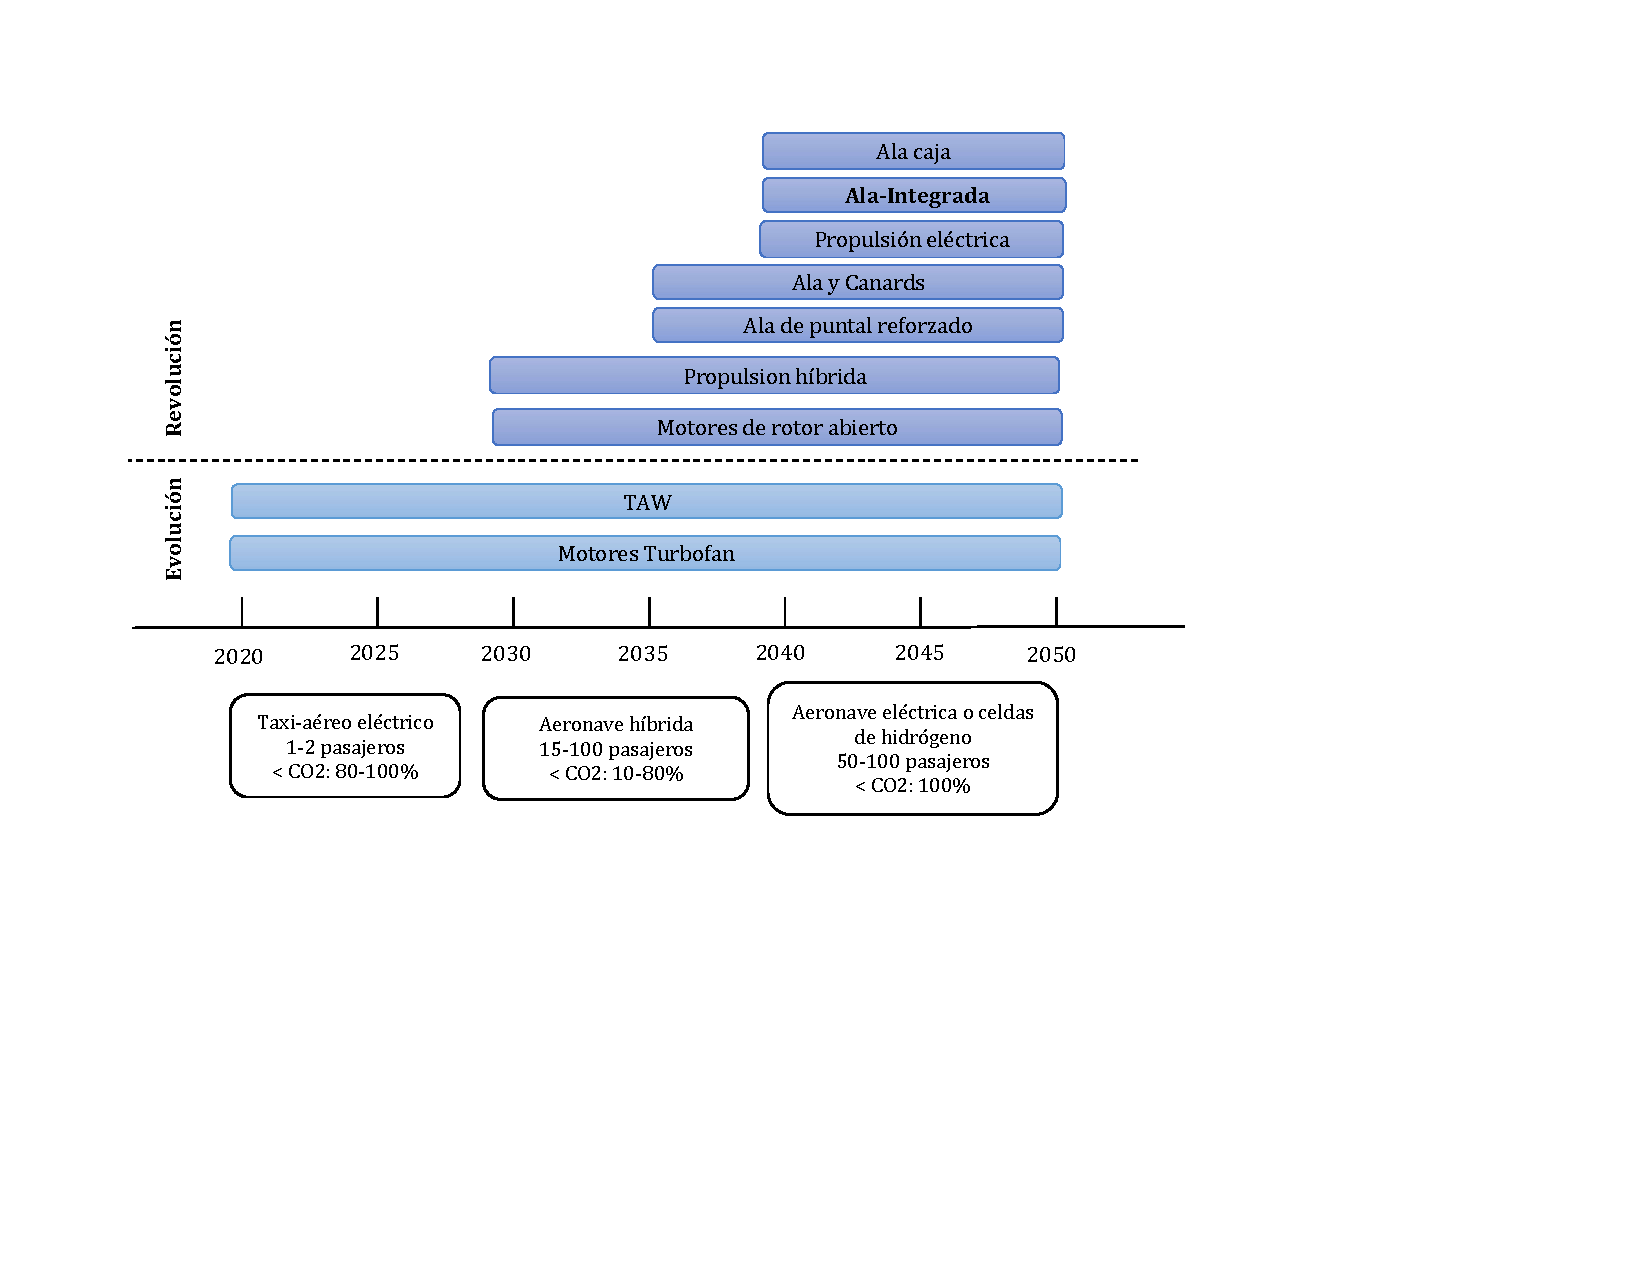
\includegraphics[scale=0.63]{Capitulo3/figs/Aviacion evolucion revolucion_cropped.pdf}
\caption{pronóstico 2020-2050 de tecnologías evolutivas y revolucionarias en la aviación \cite{IATA2020}}
\label{tecnologías evolutivas y revolucionarias}
\end{figure}
%

%%%%%%%%%%%%%%%%%%%%%%%%%%%%%%%%%%%%%%%%%%%%%%%%%%%%%%%%%%%%%%%%%%%%%%
%
Timothy Risch, líder del proyecto X-48 BWB de la NASA, considera que la aeronave de ala-integrada es una configuración de aeronave que se caracteriza por un diseño general con mínimas distinciones entre el ala y el fuselaje. Una aeronave de ala-integrada parece un ala-voladora pero concentra un mayor volumen en forma Delta en su sección central, lo suficientemente larga para una cabina de pasajeros, que está integrada dentro de los paneles del ala, ver Figura \ref{fig: configuraciones de aeronaves}. 
El pronóstico de mejora de BWB respecto a TAW en rendimiento de combustible se estima por encima del $27\%$. 
%
\begin{figure}[h]
\centering
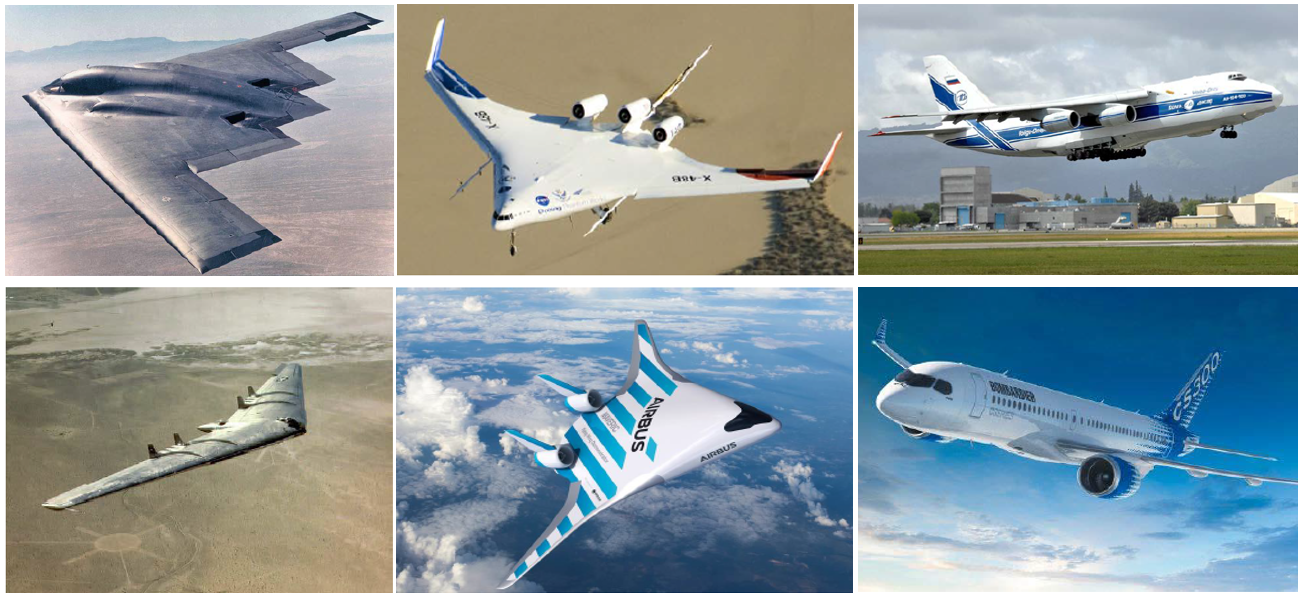
\includegraphics[scale=0.5]{Capitulo3/figs/2 5.png}
\caption{Configuraciones de aeronaves: Ala-Voladora (FW), Ala-Integrada (BWB) y Tubo-Ala (TAW)}
\label{fig: configuraciones de aeronaves}
\end{figure}
%

En \cite{IATA2020}, de acuerdo con una metodología del Centro Aeroespacial Alemán (DLR) se estima el ahorro potencial en emisiones de carbono $CO_2$ de acuerdo con distintos escenarios de implementación tecnológica:
\begin{enumerate}
    \item $T1$: Tecnologías inminentes. Mejoras evidentes en la tecnología actual próximas a lanzarse.
    \item $T2$: Tecnologías conservativas. Mejoras en motores turbofan sin cambios radicales.
    \item $T3$: Tecnologías radicales. Nuevos motores turbofan y rotores abiertos. Mejoras substanciales a las nuevas configuraciones (BWB, por ejemplo).
    \item $T4$: Tecnologías más allá. Mejoras adicionales a las nuevas configuraciones (T3), sistemas híbridos bajos en emisiones, y sistemas eléctricos y de hidrógeno libres de emisiones, energéticamente $100\%$ renovables. 
\end{enumerate}
%DLR propone 8 categorías de asientos para pasajeros: 1) 51-100, 2) 101-150, 3) 151-210, 4) 211-300, 5) 301-400, 6) 401-500, 7) 501-600, 8) 601-650. 
%
Todos los escenarios van desde un ahorro en combustible del $27\%$ hasta el $100\%$.
Las mejoras $T1,T2$ en TAW y sus motores turbofan se figuran con un impacto entre $27-45 \%$, mientras que la aeronave BWB se encuentra en los escenarios $T3,T4$ con significativas mejoras en el ahorro de combustible, teniendo la capacidad de alcanzar un $100\%$ en sus versiones eléctricas y de celdas de hidrógeno.
%
\begin{figure}[h]
\centering
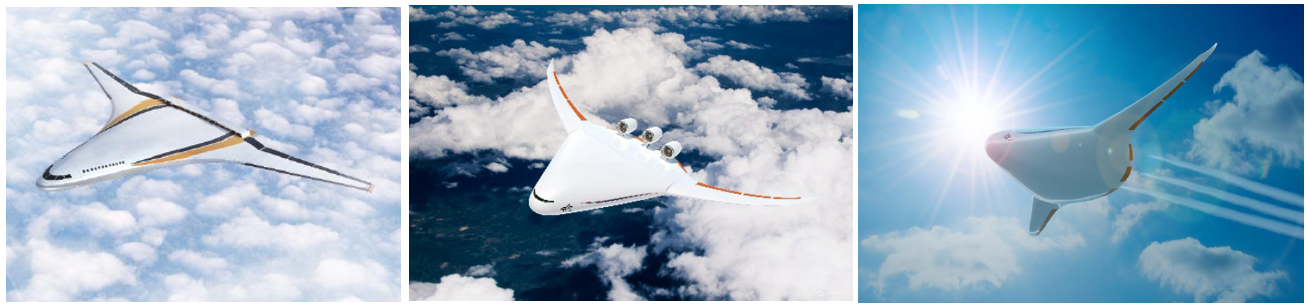
\includegraphics[scale=0.5]{Capitulo3/figs/2 3.png}
\caption{NASA-BWB turbo-eléctrico y DLR-BWB  \cite{IATA2020}}
\label{fig: NASA-BWB y DLR-BWB}
\end{figure}
%
%
Sin embargo, el diseño de una aeronave BWB requiere de una alta integración de análisis preliminares.
%%%%%%%%%%%%%%%%%%%%%%%%%%%%%%%%%%%%%%%%%%%%%%%%%%%%%%%%%%%%%%%%%%%%%%%
% Estrategias de diseño en propulsión y estructura

En \cite{Kumar2017} se presenta el diseño y el análisis de la ubicación y el número de motores para una aeronave BWB. Como resultado de este diseño se obtiene que la ubicación de los motores encima del cuerpo BWB mejora la razón levantamiento/arrastre en un $10 \%$.  Además, la base de una aeronave de ala-integrada es idónea para tener un sistema de propulsión de ingestión de la capa límite (BLI, en inglés) y/o sistemas de propulsión distribuida. Lo cual le permite mayor maniobrabilidad a costo de un control sobre-actuado.
%
\begin{figure}[!h]
\centering
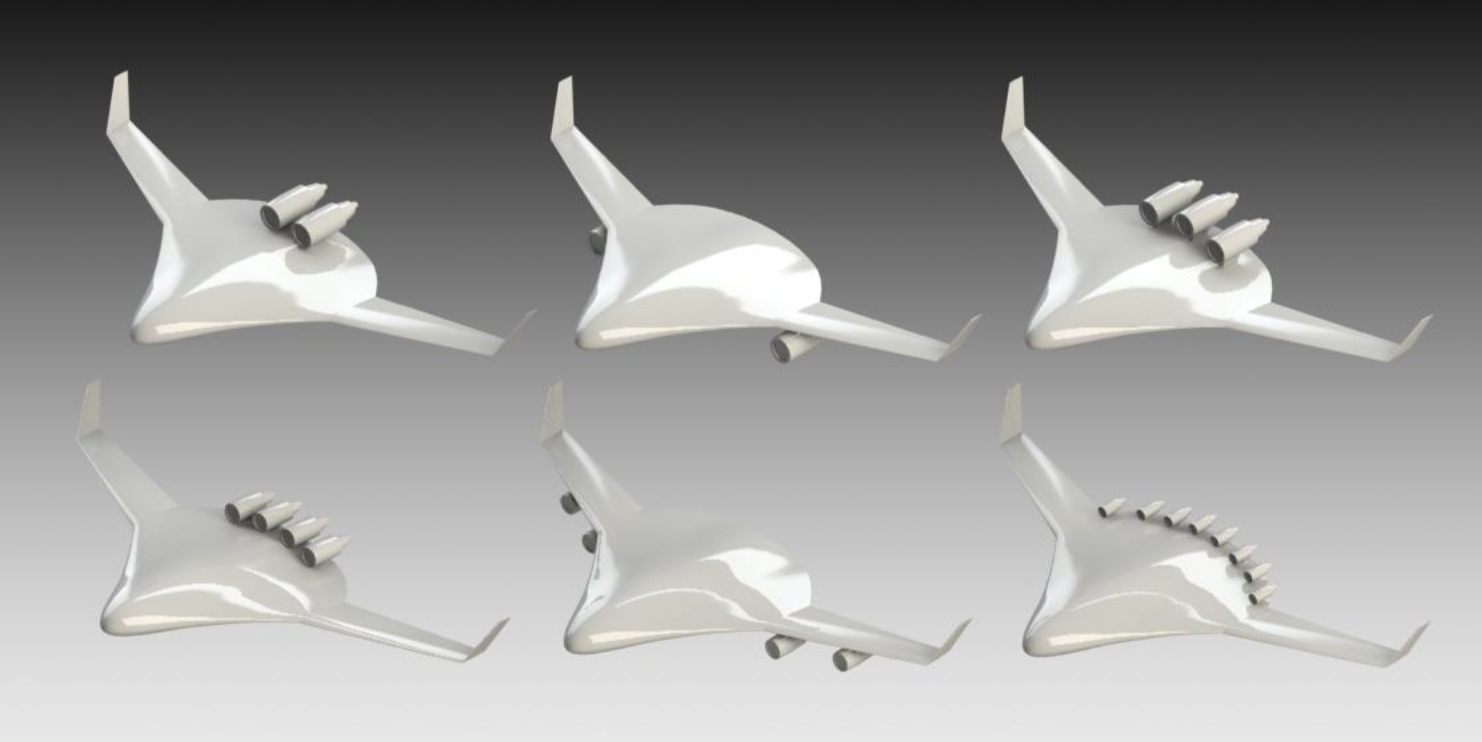
\includegraphics[scale=0.35]{Capitulo3/figs/2 4.png}
\caption{Ala-Integrada y opciones de propulsión distribuida  \cite{Kumar2017}}
\label{fig: propulsion distribuida}
\end{figure}
%
La implementación de propulsión distribuida permite implementar sistemas de control de empuje vectorial reemplazando superficies de control aerodinámicas, dado que ambos dispositivos se ubican en el borde de fuga. 
%
Adicionalmente, como parte de este trabajo se analizaron seis opciones de propulsión para BWB: 1) dos motores encima, 2) dos motores debajo, 3) tres motores encima, 4) cuatro motores encima, 5) cuatro motores debajo y 6) ocho motores encima, ver Figura \ref{fig: propulsion distribuida}. Aunque se concluyó que no existe un sistema de propulsión óptimo para BWB; se menciona que el modelo de ocho motores es el de mejor rendimiento aerodinámico, el de tres motores es ideal para el máximo peso de despegue, el de dos motores es el caso óptimo para peso vacío, y el de cuatro motores es el más eficiente en el consumo de combustible específico de empuje. 
%
En contraste, las configuraciones de tres y cuatro motores poseen una larga disrupción del flujo de aire, generando turbulencia y un aumento en el arrastre. Más motores aún de considerable tamaño (3-4 motores) decrecen el rendimiento aerodinámico.
%
Por otra parte, se sostiene que tanto dos como ocho motores son la promesa del futuro para BWB, pero al mismo tiempo, el autor apuesta aún más por la propulsión de ocho motores dados su mejores resultados en razón levantamiento/arrastre, rendimiento aerodinámico y menor peso máximo de despegue; en contraste con la peor opción en el consumo de combustible específico. 
%
Dado que el análisis utilizó motores existentes, se plantea que motores diseñados para una aeronave BWB particular, con nuevos materiales y tecnología puede hacer de la configuración de ocho motores la más eficiente en esta configuración. Sin embargo, en espera de esa tecnología la localización de dos motores sería la opción más viable con mejor rendimiento. 


En \cite{Panagiotiu2017}, se estudia el diseño aerodinámico de aeronaves BWB no tripuladas para seleccionar la combinación estructural óptima donde el principal objetivo es conseguir tanto el rendimiento como la estabilidad aerodinámica y el control.
%
\begin{figure}[!h]
\centering
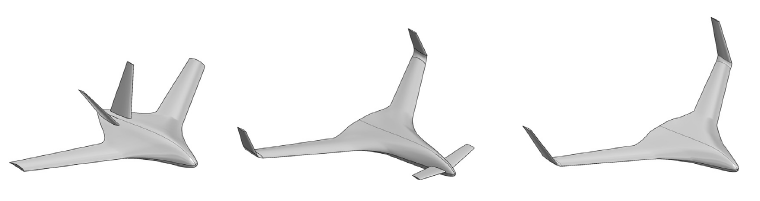
\includegraphics[scale=0.8]{Capitulo3/figs/2 9.png}
\caption{Configuraciones BWB para aerodinámica y control: 1) Estabilizador vertical en V, 2) Canards y 3) Aletas en punta \cite{Panagiotiu2017}}
\label{fig: configuraciones BWB aero y control}
\end{figure}
%
Se proponen tres configuraciones para la estabilidad y el control: 1) estabilizadores verticales en V para la estabilidad y el control longitudinal y direccional, 2) canards para estabilidad y control longitudinal y 3) aletas en las puntas para estabilidad y control direccional, ver Figura \ref{fig: configuraciones BWB aero y control}. 
%
Las tres configuraciones cuentan con elevons en el borde de fuga para generar los momentos de cabeceo y alabeo. 
Si bien las tres configuraciones proporcionan buenas métricas dado un bajo arrastre y una alta razón levantamiento/arrastre, el modelo 3) presenta el mejor coeficiente de levantamiento. 
La configuración 1) sería el modelo menos eficiente en aerodinámica, dado el arrastre generado por la estabilizadores en V. 
%
En términos de estabilidad, dada la gran capacidad que tenemos en el volumen interno, es posible localizar el centro de gravedad donde mejor convenga. Asimismo deben seleccionarse perfiles aerodinámicos que permitan adecuar el volumen interno de la carga útil y los sistemas de la aeronave como los tanques, celdas o baterías de energía.
%
Perfiles aerodinámicos con comba son empleados para propósitos de estabilidad longitudinal, buscando reducir el momento de cabeceo hacia abajo, que de no atenderlo, incrementarían los requerimientos para el \textit{trimming} o vuelo en equilibrio, lo que a su vez genera mayor arrastre y consumo energético de las entradas de control. 

\medskip

De acuerdo con \cite{CHEN2019}, es posible mencionar los siguientes \textbf{Beneficios de BWB}:
\begin{itemize}
    \item Reducción del arrastre de fricción por una menor área de contacto con el fluido considerando un mismo volumen, el arrastre de compensación puede evitarse adoptando una estabilidad relajada en el cabeceo, reducción del arrastre de interferencia gracias a una armonioso ensamble cuerpo central-ala, reducción del arrastre inducido por sustentación gracia a una distribución de levantamiento en todo el vehículo, reducción del arrastre de olas a velocidad transónica debido a una mejor morfología aerodinámica., simplificación en los dispositivos hiper-sustentadores, en la reducción del peso de ala y un mejor margen a alta-altitud gracias a la reducción de la carga alar, permite la ubicación de los motores encima del cuerpo central lo que reduce significativamente el ruido producido, el alivio de la carga aerodinámica local mediante la carga de inercia local puede reducir las cargas de flexión y de corte en la estructura, la simplicidad de la configuración sugiere una reducción en los costos de manufactura. Además, BWB es una configuración ideal para tecnología de flujo laminar, configuración ajustable para aplicaciones de alta capacidad y reducción significativa de costos en operaciones directas pueden lograrse.
\end{itemize}
%\begin{itemize}
%    \item Reducción del arrastre de fricción por una menor área de contacto con el fluido considerando un mismo volumen.
%    \item El arrastre de compensación puede evitarse adoptando una estabilidad relajada en el cabeceo.
%    \item Reducción del arrastre de interferencia gracias a una armonioso ensamble cuerpo central-ala.
%    \item Reducción del arrastre inducido por sustentación gracia a una distribución de levantamiento en todo el vehículo.
%    \item Reducción del arrastre de olas a velocidad transónica debido a una mejor morfología aerodinámica.
%    \item Simplificación en los dispositivos hiper-sustentadores, en la reducción del peso de ala y un mejor margen a alta-altitud gracias a la reducción de la carga alar. 
%    \item Permite la ubicación de los motores encima del cuerpo central lo que reduce significativamente el ruido producido.
%    \item El alivio de la carga aerodinámica local mediante la carga de inercia local puede reducir las cargas de flexión y de corte en la estructura.
%    \item La simplicidad de la configuración sugiere una reducción en los costos de manufactura.
%    \item Configuración ideal para tecnología de flujo laminar.
%    \item Configuración ajustable para aplicaciones de alta capacidad. 
%    \item Reducción significativa de costos en operaciones directas pueden lograrse.
%\end{itemize}
%
Asimismo, algunos \textbf{Retos de BWB} o problemas abiertos son:
\begin{itemize}
    \item Requiere una estabilidad estática relajada y un \textbf{sistema de control de vuelo automático} para volar eficientemente, penalización en el peso debido a una cabina no circular presurizada, cualidades de vuelo y de maniobra inferiores debido a una estabilidad relajada, autoridad de control limitada y un complejo diseño del sistema de control de vuelo, capacidad de recuperación para caídas potenciales en aeronaves sin empenaje, menor número de ventanillas reflejado en menor confort para los pasajeros en vuelos comerciales, satisfacer los requerimientos de evacuación y certificados de navegabilidad, sensibilidad a las ráfagas de viento debido a una menor carga alar, limitaciones en la infraestructura actual para modelos a gran escala debido a las calles de rodaje y pista diseñadas para el uso de modelos TAW, diseño total de un nuevo sistema de propulsión integrada, posible diseño e integración de un sistema de flujo laminar, manufactura de componentes muy grandes (probablemente materiales compuestos) y aeroeslasticidad.
\end{itemize}

%\begin{itemize}
%    \item Requiere una estabilidad estática relajada y un \textbf{sistema de control de vuelo automático} para volar eficientemente.
%    \item Penalización en el peso debido a una cabina no circular presurizada.
%    \item Cualidades de vuelo y de maniobra inferiores debido a una estabilidad relajada, autoridad de control limitada y un complejo diseño del sistema de control de vuelo. 
%    \item Capacidad de recuperación para caídas potenciales en aeronaves sin empenaje.
%    \item Menor número de ventanillas reflejado en menor confort para los pasajeros en vuelos comerciales.
%    \item Satisfacer los requerimientos de evacuación y certificados de navegabilidad.
%    \item Sensibilidad a las ráfagas de viento debido a una menor carga alar.
%    \item Limitaciones en la infraestructura actual para modelos a gran escala debido a las calles de rodaje y pista diseñadas para el uso de modelos TAW.
%    \item Diseño total de un nuevo sistema de propulsión integrada.
%    \item Posible diseño e integración de un sistema de flujo laminar.
%    \item Manufactura de componentes muy grandes (probablemente materiales compuestos).
%    \item Aeroeslasticidad.
%\end{itemize}

%%%%%%%%%%%%%%%%%%%%%%%%%%%%%%%%%%%%%%%%%%%%%%%%%%%%%%%%%%%%%%%%%%%%%
\section{Origen de BWB}

De acuerdo con Bruce I. Larrimer en \cite{Larrimer2020}, en el verano de 1988 Dennis Bushell de NASA invitaba a través de cartas a representantes de McDonnell Douglas, ingenieros aeronáuticos y aerodinámistas al Centro de Investigaciones Langley de la NASA (LaRC), para atender y resolver la siguiente pregunta: \textit{¿Cabe lugar para un transporte aéreo de gran capacidad y largo alcance que genere un renacimiento aerodinámico?}. 
\begin{figure}[!h]
\centering
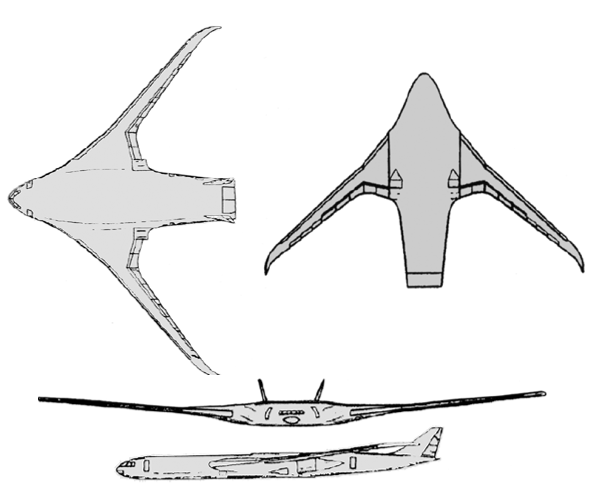
\includegraphics[scale=0.72]{Capitulo3/figs/2 6.png}
\caption{Siguiendo la primera conceptualización de BWB, Liebeck y sus colegas de McDonnell Douglas generaron la configuración de transporte (primera generación) en prototipo. Esta sirvió de base para propuestas posteriores como BWB-450 después X-48B de NASA \cite{Larrimer2020}}
\label{fig: primer concepto de Ala-Integrada}
\end{figure}
%
Bushnell cuestionaba principalmente el paso evolutivo en el diseño de aeronaves de transporte, resaltando que el desarrollo revolucionario como el Boeing 707 y Douglas DC 8, la primera generación de jets de ala en flecha que revolucionó el comercio aéreo internacional, habían sido exitosos por diseños que siguen una línea cautelosa, incremental y de patrón evolutivo. 
%
En la primavera de 1989 casi dos docenas de líderes gubernamentales y de la industria junto con académicos e ingenieros aeronáuticos y aerodinámistas se reunieron en el LaRC de la NASA para discutir posibles nuevas configuraciones de aeronaves. 
%
%\begin{itemize}
%    \item Preparar una aeronave como matriz de referencia\footnote{Sistema de coordenadas que se utiliza para definir la orientación y posición de montajes de componentes, distribución de cargas, ubicación de sistemas y otros aspectos de diseño, esenciales para la simulación y análisis de vuelo de aeronaves.} de acuerdo con la configuración TAW nombrada Transporte de Tecnología Sinérgica (\textit{Sinergistic Technology Transport ó STT n en inglés}) que sirva de base para unificar las filosofías de evolución y revolución en el diseño de aeronaves. 
%    \item A partir de la aeronave base \textit{STT}, proponer un diseño revolucionario con técnicas de optimización sin limitaciones
%    \item Comparar los resultados de aproximación de los dos diseños
%\end{itemize}
%
La matriz de referencia\footnote{Sistema de coordenadas que se utiliza para definir la orientación y posición de montajes de componentes, distribución de cargas, ubicación de sistemas y otros aspectos de diseño, esenciales para la simulación y análisis de vuelo de aeronaves.} de acuerdo con la configuración TAW fue nombrada Transporte de Tecnología Sinérgica (Sinergistic Technology Transport ó STT n en inglés) con el objetivo de unificar las filosofías de evolución entre los modelos de aeronaves DC-10 y MD-11. Robert H.Liebeck junto a sus colegas de McDonnell Douglas presentaron la aeronave de ala-integrada como propuesta de evolución y revolución, ver Figura \ref{fig: primer concepto de Ala-Integrada}.
Las características de la misión de vuelo para el análisis comparativo entre STT y el primer concepto BWB fueron un rango de operación de 8,500 millas náuticas con una capacidad para 368 pasajeros viajando a una velocidad crucero de 0.85 Mach.
Los resultados demostraron un amplia mejora en el primer concepto BWB sobre el STT, obteniendo un razón levantamiento/arrastre de 33.3 sobre 23.1, lo que resultó en un ahorro de combustible del 25.7 $\%$, \cite{Larrimer2020}.
%
Robert H.Liebeck concluyó su estudio con la siguiente nota: \textit{la aeronave que resulta de ambos conceptos (evolución y revolución) ofrece mejoras de rendimiento tales sobre las aeronaves existentes que respondemos a la pregunta de la NASA con un definitivo SI}.
%
Este fue el inicio del reconocible esfuerzo en el diseño, desarrollo y pruebas de prototipos en túnel de viento y pruebas de vuelo del concepto BWB.


%En la Tabla \ref{tab: STT vs BWB} podemos observar la significativa optimización del concepto revolucionario de una aeronave de ala-integrada sobre la matriz de referencia \textit{STT} como concepto evolutivo. 
%
%\begin{table}[!h]
%\caption{STT comparado con BWB\cite{Larrimer2020}}
%\label{tab: STT vs BWB}
%\centering
%\begin{tabular}{ |p{4.5cm}||p{2cm}|p{2cm}|}
% \hline
% Características & STT & BWB \\
% \hline
% Diseño en millas nauticas & 8,500 & 8,500 \\
% Pasajeros & 368 & 368  \\
% Mach en crucero & 0.85 &  0.85 \\
% Motores & 3 VHBR & 2 VHBR \\
% Empuje (c/u) & 30,600 lb & 30,900 lb\\
% Envergadura & 188 ft & 260 ft \\
% Largo & 236 ft & 167  ft \\
% Área de ala & 2,020 $ft^2$ & 4,500 $ft^2$ \\
% Peso total & 367,200 lb & 338,800 lb\\
% Peso vacio operativo & 192,700 lb & 195,300 lb \\
% Levantamiento/Arrastre & 23.1 & 33.3\\
%Ahorro en combustible & base & 25.7 $\%$\\
% \hline
%\end{tabular}
%\end{table}
%


%%%%%%%%%%%%%%%%%%%%%%%%%%%%%%%%%%%%%%%%%%%%%%%%%%%%%%%%%%%%%%%%%%%
% Historia. líneas de tiempo y desarrollos BWB.

A partir de los esfuerzos en conjunto de NASA, McDonnell Douglas y del principal pionero en la configuración BWB, Liebeck, se reveló el enorme potencial de BWB para satisfacer las necesidades ecológicas de las aerolíneas. 
%
La Tabla \ref{tab: Desarrollos BWB en el mundo} muestra los principales desarrollos BWB de USA,Europa, Rusia y China. Algunas de las aeronaves BWB estudiadas se muestran en la Figura \ref{fig: evolucion de BWB}.  
%
El último modelo BWB de USA desarrollado para pruebas de vuelo fue el \textbf{X-48C}. Sus antecesores X-48 y X-48B fueron desarrollados para pruebas en túnel de viento y pruebas de vuelo, respectivamente. 
%
Por parte de USA, desde el origen de BWB continuaron con su investigación con los proyectos de BWB-tech. Más tarde, McDonnell Douglas se hacia parte de Boeing y evolucionaría en el proyecto de pruebas de vuelo para el modelo \textbf{X-48B}.
\begin{figure}[!h]
\centering
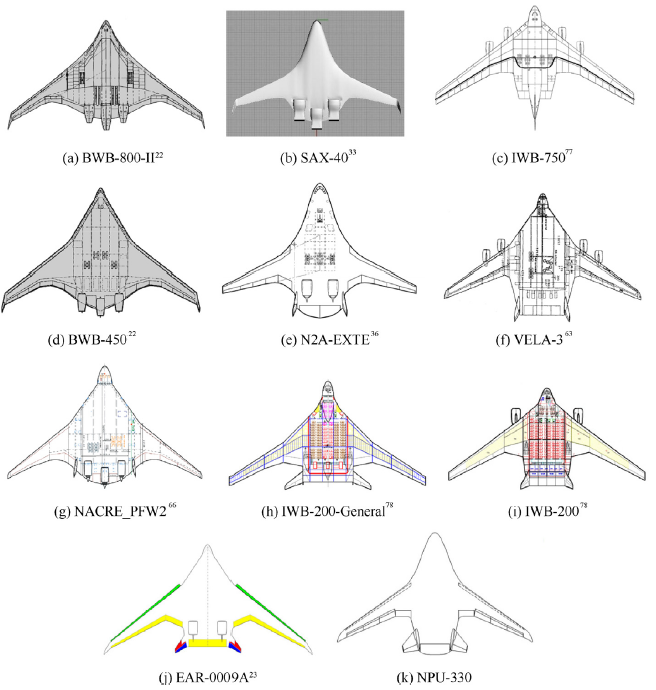
\includegraphics[scale=0.8]{Capitulo3/figs/2 7.png}
\caption{ Evolución del concepto de Ala-Integrada BWB \cite{CHEN2019}}
\label{fig: evolucion de BWB}
\end{figure}

\begin{table}[!t]
\caption{Desarrollo de Aeronaves BWB en USA,Europa,Rusia y China \cite{CHEN2019}}
\label{tab: Desarrollos BWB en el mundo}
\centering
\begin{tabular}{ |p{1.9cm}|p{2.2cm}|p{2.5cm}|p{1.8cm}|p{1.9cm}|p{1.6cm}|  }
\hline
\multicolumn{6}{|c|}{Desarrollo de aeronaves BWB} \\
\hline
Año & Proyecto & BWB-Nombre & Pasajeros & Rango(km) & Mach \\
\hline
\multicolumn{6}{|c|}{Principales proyectos BWB en USA} \\
\hline
1994-1997 & BWB-tech & BWB-800-II & 800 & 13,000 & 0.85 \\
1997-2002 & Boeing & BWB-450 & 478 & 14,400 & 0.85 \\
2002-2012 & Flight test & X-48B & UAV & - & - \\
2003-2006 & SAI & SAX-40 & 215 & 9,300 & 0.8 \\
2007-2011 & SFW & N2A-EXTE & 262 & 11,100 & 0.8 \\
2010-2015 & ERA & ERA-0009A & 224 & 14,800 & 0.85   \\
2012-2013 & Flight test & X-48C & UAV & - & - \\
\hline
\multicolumn{6}{|c|}{Principales proyectos BWB en Europa} \\
\hline
1998-2002 & Cranfield & BWB-98 & 960 & 14,200 & 0.85 \\
2000-2003 & MOB & BWB-MOB & - & - & 0.85 \\
2002-2005 & VELA & VELA-3 & 750 & 14,200 & 0.85 \\
2005-2010 & NACRE & NACRE & 750 & 14,200 & 0.85 \\
2008-2011 & ACFA2020 & ACFA-2020 & 470 & 13,300 & 0.85 \\
2015-2018 & AGILE & AGILE-BWB & 450 & 15,700 & 0.85 \\
2012-now & Airbus future & Airbus BWB & 470 & 13,300 & 0.85 \\
\hline
\multicolumn{6}{|c|}{Principales proyectos BWB en Rusia} \\
\hline
1997-2001 & 548-97 ISTC & IWB-750 & 750 & 13,700 & 0.85 \\
2014 &   & FW-200 & 211 & 16,000 & 0.85 \\
2019 &  & BWB-325 & 325 & 12,550 & 0.85 \\
\hline
\multicolumn{6}{|c|}{Principales proyectos BWB en China} \\
\hline
2008-2017 & BWB & NPU-330 & 330 & 13,900 & 0.85 \\
\hline
\end{tabular}
\end{table}


%Los proyectos SAI, SFW y ERA proponían objetivos específicos en la investigación de BWB.
%Las siglas en inglés SAI refieren a la iniciativa para una \textbf{aeronave silenciosa}, dónde se implemento un sistema de propulsión de ingestión de la capa límite. 
%Las siglas en inglés SFW refieren a una aeronave subsónica de ala-fija. La intención con este proyecto era probar una aeronave híbrida BWB en túnel de viento que \textbf{minimizará la contaminación de ruido y emisiones}. 
%Las siglas en inglés ERA refieren a una \textbf{aviación ambientalmente responsable}, con el objetivo de minimizar el ruido, las emisiones y la quema de combustible para 2025.
%
%Poco después de que USA mostrará el potencial increíble de BWB, la Unión Europea comenzó sus propios desarrollos. El primer concepto que diseñaron era similar al propuesto por Boeing, y fue estudiado por la universidad de Cranfield. El diseño y desarrollo para aeronaves BWB fue progresivo y una sinergia entre distintos países de la Unión Europea, principalmente Francia y Alemania. 
%
%Por su parte, Rusia colaboró con USA y Europa para sus primeras conceptos de BWB, sustentados por el Centro Científico y Técnico Internacional (ISTC, en inglés) dónde lanzó IWB-750 de gran capacidad. %Las siguientes propuestas fueron para aeronaves más pequeñas. 
%
%Asimismo, China lanzó su investigación relativamente tarde, en 2008, dónde su primer versión fue para una capacidad de 150 pasajeros. Las siguiente versión fue para 300 pasajeros hasta llegar a su última versión propuesta para 330 pasajeros. 
%
%De acuerdo a lo anterior podemos concluir que desde el origen de BWB en USA, la investigación y desarrollo se ha llevado a cabo en sinergia entre USA y Europa principalmente. 


%%%%%%%%%%%%%%%%%%%%%%%%%%%%%%%%%%%%%%%%%%%%%%%%%%%%%%%%%%%%%%%%%%%%%%%%%%
% Prototipos para pruebas en túnel de viento y pruebas de vuelo

\section{Modelos a escala - bancos de pruebas}

La investigación en modelos a escala de aeronaves juega un papel fundamental en el desarrollo de nuevas configuraciones en escala real, siendo herramientas poderosas para explorar la envolvente de vuelo. 
Algunos modelos a escala para pruebas en túnel de viento y pruebas de vuelo se muestran en la Figura \ref{fig BWB prototipos}. 
%
\begin{figure}[h]
\centering
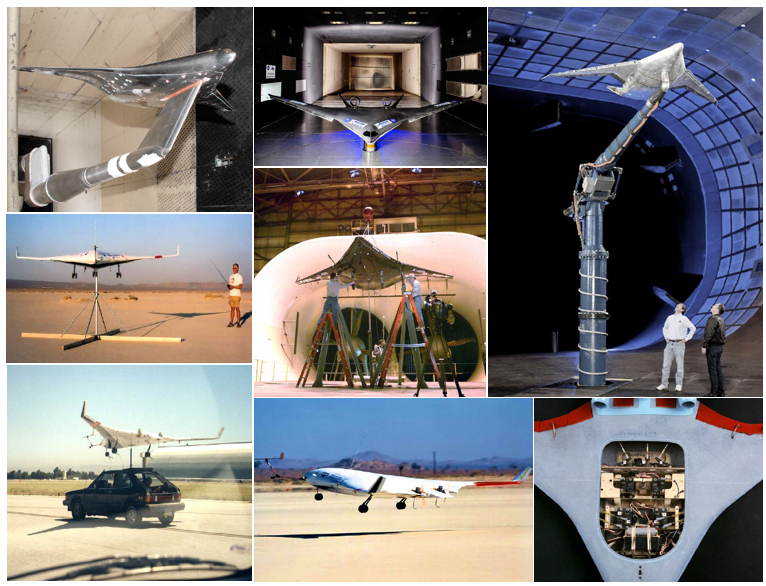
\includegraphics[scale=0.8]{Capitulo3/figs/2 8.png}
\caption{Modelos a escala de túnel de viento y pruebas de vuelo y control \cite{Larrimer2020}}
\label{fig BWB prototipos}
\end{figure}
%
Ahora en 2023, las principales compañías manufactureras de aeronaves Boeing y Airbus después de treinta años de investigación y desarrollo en el modelo de aeronave BWB poseen un avance substancial en lo que figura ser las primeras aeronaves BWB candidatas para vuelos comerciales como el X-48 B/C y MAVERIC, respectivamente. 

%%%%%%%%%%%%%%%%%%%%%%%%%%%%%%%%%%%%%%%%%%%%%%%%%%%%%%%%%%%%%%%%
% MAVERIC and X-48
%

\medskip


\textbf{Boeing X-48 B/C}\footnote{El reto era evaluar la mecánica de vuelo del concepto BWB y probar que podemos mantener la estabilidad y el control. Abordamos exhaustivamente estos problemas con X-48B y obtuvimos excelentes resultados. \textit{Robert H. Liebeck}.} 

%\textit{El reto era evaluar la mecánica de vuelo del concepto de Ala-integrada y probar que podemos mantener la estabilidad y el control. Abordamos exhaustivamente estos problemas con X-48B y obtuvimos excelentes resultados.} \textit{Robert H. Liebeck}. 
%
\begin{figure}[h]
\centering
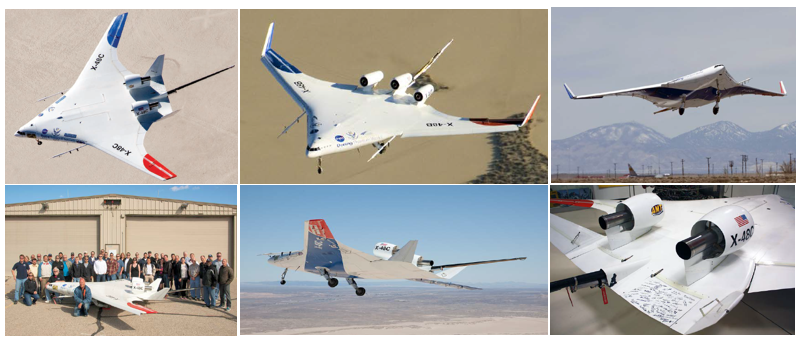
\includegraphics[scale=0.8]{Capitulo3/figs/2 10.png}
\caption{ Boeing X-48 B/C BWB \cite{Larrimer2020}}
\label{fig: Boeing X-48}
\end{figure}
%
%
La aeronave \textbf{BWB X-48B} es un prototipo a escala al 8.5\% de la versión de Boeing BWB-450-1L con una envergadura de 73m. 
El modelo a escala tiene la misma distribución en peso que el modelo real y permite simulaciones con los mismos momentos de inercia y coeficientes de fuerza aerodinámica, lo que permite validar la estabilidad y el control como cualidades de maniobra. 
%Algunas características son:
%
%\begin{itemize}
%    \item Motores y sistema de combustible. Tres motores de gas turbofan JetCat USA P200 y una unidad de control de motores (ECUs). Cada motor produce 24.5kg de empuje a nivel del mar. Cada motor tiene su propio control de aceleración, de circuito de combustible y de bombeo de combustible. El tanque de gasolina de 47L permite una autonomía de 30-35min.   
%    \item Sistema eléctrico. 2 baterías de 32V y una de 6V. Una batería de 32V alimenta el subsistema de aviónica, incluyendo las computadoras de control de vuelo, el GPS y la unidad de medidas de inercia. La otra batería de 32V alimenta el sistema de actuadores excepto el timón que es alimentado por la batería de 6V. 
%    \item Sistema de navegación. Dos unidades de GPS. Uno mezclado con una unidad de medidas de inercia (IMU) para proveer altitud e información de navegación, y el independiente para proveer datos de posicionamiento. 
%    \item Aviónica y sensores. Se usaron sensores de alta calidad como un receptor de comando y un transmisor de enlace descendente de telemetría operados en el espectro de frecuencia de banda L. Una cámara en la nariz y un receptor de audio retransmitido en banda S. Un transponedor como identificador de posición para el tráfico aéreo. 20 sensores para las superficies de control conectados a la computador de control de vuelo. Dos booms de datos de aire miden la presión total, la presión estática, la temperatura estática y el ángulo de ataque como el ángulo de derrape. Un altímetro láser cambia las leyes de control de vuelo durante el despegue y aterrizaje, además de proveer lecturas de sobre el suelo con un altitud menor a 22m. Un IMU provee una alta precisión en tiempo real en posición y orientación con un sistema de navegación basado en datos GPS. Se añadió un segundo GPS. 
%\end{itemize}
%
%El modelo \textbf{X-48C} regresó a NASA DFRC en Octubre de 2009 después de un prototipo para túnel de viento en NASA Langley dónde se revisaron las modificaciones en estabilidad y control respecto a la versión X-48B. 
%
Las principales modificaciones en la versión X-48C respecto la versión X-48B fueron: eliminar las aletas con timones en la punta y reemplazarlos con un par de estabilizadores verticales en la plataforma adyacente donde se ubican los motores. Se reemplazaron los tres motores por un par de motores de gas turbofan AMT Titan de 80kg de empuje, y la plataforma adyacente donde se localizan los dos motores y los estabilizadores verticales. 
%
También se hicieron modificaciones en el controlador de vuelo anticipando las cualidades de maniobra e incluyendo restricciones del controlador de vuelo para manter la aeronave en una envolvente de vuelo segura. 
%
Para realizar las mejoras del X-48B al X-48C Boeing recibió de NASA 5.29 millones de dólares para una investigación de un año con el propósito de identificar los conceptos necesarios para que el modelo BWB pudiera entrar en servicio en el año 2025, volando con menor emisión de ruido, gases y contaminantes y menor consumo de combustible. 
%
Al concepto BWB X-48C se le nombró como aeronave híbrida de ala-fuselaje (HWB) y su objetivo específico era ser la aeronave del futuro para reducir la quema de combustible en un 50\%, con 50\% menos de emisiones contaminantes y un 83\% de menos ruido. 
%

\medskip

\textbf{Airbus MAVERIC\footnote{BWB MAVERIC viene de las siglas en inglés que significan: "Modelo de Aeronave para la Validación y Experimentación de Controladores Innovadores Robustos".}}\\
Airbus lanzó MAVERIC en 2017, comenzando sus primeras pruebas de vuelo en 2019 y continuando hasta finales del 2020. La versión a escala tiene un largo de 2m con una envergadura de 3.2m. 
%BWB MAVERIC viene de las siglas en inglés que significan: "Modelo de Aeronave para la Validación y Experimentación de Controladores Innovadores Robustos". 
%
Aunque Airbus mencionó que no tienen un tiempo específico para que su aeronave BWB entre en servicio, están firmemente convencidos que esta nueva arquitectura para vuelos comerciales será el futuro para un ambiente sustentable en la aviación. 
La propuesta MAVERIC BWB de Airbus se basa en una propulsión híbrida de baterías eléctricas y celdas de hidrógeno con el fin de asegurar cero emisiones. 
\begin{figure}[h]
\centering
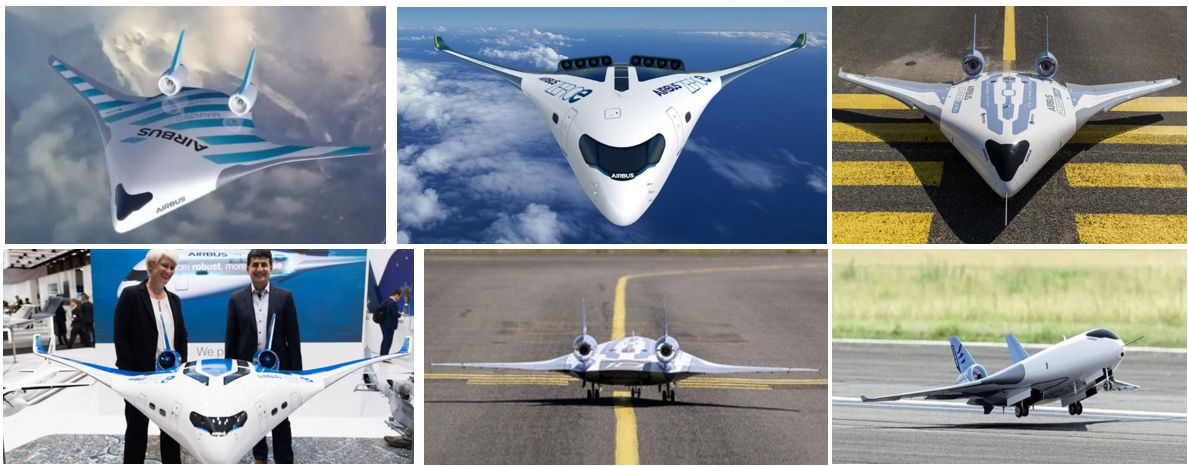
\includegraphics[scale=0.56]{Capitulo3/figs/2 11.png}
\caption{ Airbus MAVERIC BWB}
\label{fig: Airbus MAVERIC}
\end{figure}
%
%%%%%%%%%%%%%%%%%%%%%%%%%%%%%%%%%%%%%%%%%%%%%%%%%%%%%%%%%%%%%%%%%%%%%%%%%%
%%%% Ventajas/Desventajas BWB


%%%%%%%%%%%%%%%%%%%%%%%%%%%%%%%%%%%%%%%%%%%%%%%%%%%%%%%%%%%%%%%%%%%%%%%%%%%
\section{Sistemas de Control de Vuelo (FCS)}
%%%%%%%%%%%%%%%%%%%%%%%%%%%%%%%%%%%%%%%%%%%%%
%
Un Sistemas de Control de Vuelo\footnote{,Flight Control System, FCS en sus siglas en inglés}, es un conjunto de dispositivos y programas que se utilizan para controlar la trayectoria, movimiento y estabilidad de vehículos aéreos. 
%
En general, el FCS es responsable de mantener la estabilidad y control incluso en condiciones adversas de viento, turbulencias, fallas y otros factores. 
%
El FCS para aeronaves de ala-integrada debe incluir las siguientes especificaciones:
\begin{itemize}
    \item  Sistema de Control de Vuelo Digital con Total-Autoridad Fly-By-Wire (DFBW). La configuración BWB no tiene las superficies de control aerodinámicas en los estabilizadores horizontales y verticales de un empenaje, y por lo tanto, debe fiarse de un sistema de control de vuelo digital con total-autoridad fly-by-wire (DFBW) para estabilidad, control y rutina de vuelo en equilibrio. 
    El DFBW puede trabajar en sinergia con un esquema de asignación de control para minimizar las velocidades de los actuadores, las fuerzas requeridas de las ACS y los requerimientos de poder de todas las entradas de control.
    \item Sensores. Los FCS están equipados con una variedad de sensores para medir la velocidad, la altitud, la dirección, la aceleración, la temperatura y otros parámetros de la aeronave. Estos sensores también incluirían giroscopios y acelerómetros para medir la orientación y la inclinación de la aeronave. 
    \item Actuadores. Los mecanismos que accionan los efectores de control se llaman actuadores.  Los modelos BWB cuentan con un número mayor de efectores de control, y por tanto de actuadores. Los actuadores están conectados a las superficies de control aerodinámicas y a los mecanismos de la tobera de empuje vectorial.
    \item Sistema de Navegación. Utiliza señales de satélite para determinar la posición y la trayectoria de la aeronave, así como un sistema de comunicación que permite la transmisión de datos entre la aeronave y los controladores de tráfico aéreo. 
    \item Software. El FCS incluye software avanzado que realiza cálculos complejos y toma decisiones en tiempo real para mantener la estabilidad y control del vehículo aéreo.
\end{itemize}
%
En un análisis inicial de las características aerodinámicas del BWB se identificó una falla potencial en sus giros sostenidos y modos posteriores a la salida con el morro hacia arriba; ambas preocupaciones históricas con las aeronaves de ala-voladora y sin empenaje. Este tipo de amenazas son de extrema importancia. El comportamiento potencial de una aeronave BWB tiene que evaluarse en los bordes de los niveles de baja y alta velocidad de la envolvente, incluido el comportamiento de entrada en pérdida, así como posibles caídas, picadas y golpes (una combinación de todos estos ha destruido aeronaves Northrop YB-49A décadas anteriores).

\bigskip

%%%%%%%%%%%%%%%%%%%
\textbf{X-48 B/C}\\
La NASA emprendió investigaciones de vuelo con las aeronaves X-48B y X-48C en el Centro de Investigación de Vuelo Dryden de la NASA (DFRC) entre el 20 de julio de 2007 y el 9 de abril de 2013. Ambas versiones de vehículos completaron un total de 122 vuelos piloteados remotamente (92 vuelos con X-48B y 30 vuelos con X-48 C). La duración de cada vuelo fue en un rango entre 30-35 minutos. 
X-48B cuenta con 20 ACS acopladas como efectores de control para los momentos de cabeceo, alabeo y guiñada, ver Figura \ref{fig: Boeing X-48B ACS}. 
\begin{figure}[!h]
\centering
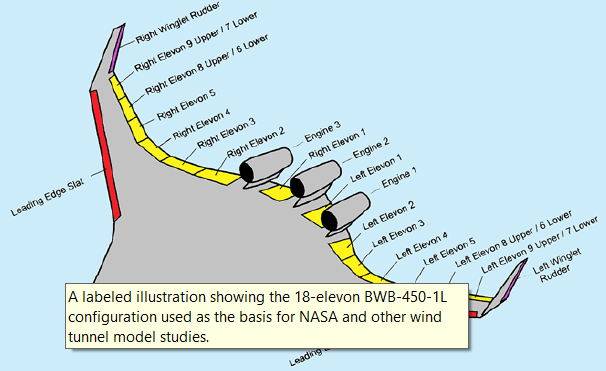
\includegraphics[scale=0.8]{Capitulo3/figs/2 23.png}
\caption{ Boeing X-48B con Superficies de Control Aerodinámicas \cite{Larrimer2020}}
\label{fig: Boeing X-48B ACS}
\end{figure}
X-48B tiene un par de elevadores entre sus tres motores, cuatro pares de elevons para la combinación de cabeceo y guiñada, y dos pares de timones de arrastre que puede actuar como alerones o frenos de velocidad. Las aletas en la punta del ala sirven como estabilizadores verticales y cuentan con timones de dirección.
%
%El programa de prueba de vuelo fue un esfuerzo hecho por NASA, la Fuerza Aérea de Estados Unidos, la compañia Boeing y Cranfield Aerospace. 
%
%La evaluación del programa de pruebas de vuelo para el X-48B buscó demostrar limitadores robustos del ángulo de ataque y deslizamiento lateral que proporcionarán resistencia de salida y permitieran maniobras agresivas hasta el $C_{Lmax}$ y un límite de deslizamiento lateral equivalente a un aterrizaje normal a gran escala en un viento cruzado de 35 nudos. 
%
En \cite{Larrimer2020} pueden encontrarse las tablas de los seis bloques de las pruebas de vuelo de X-48B y X-48C, dónde se observa el uso de controladores PID principalmente, entre algunos otros. 
%
Para X-48 B/C tres sistemas aumentados independientes (cabeceo, alabeo y guiñada) trabajan en conjunto el control por asignación:
\begin{itemize}
    \item Sistema aumentado de control y estabilidad longitudinal (LSCAS)
    \item Sistema aumentado de control y estabilidad de alabeo (RSCAS)
    \item Sistema aumentado de control y estabilidad de guiñada (DSCAS)
\end{itemize}
%
Una deficiencia en cualquier ley de control comprometería las operaciones y la estabilidad del sistema completo.
Por ejemplo, una demanda mayor de energía de la disponible provocaría que no contar con la suficiente deflexión de las ACS. 
%
%Las actividades que se esperan lograr mediante \textbf{asignación de control} en X-48 B/C son las siguientes: 
%\begin{itemize}
    %\item Comandar las ACS obteniendo los momentos desacoplados de cabeceo, alabeo y guiñada demandados por el sistema de aumentado de estabilidad y control.
    %\item Generar las aceleraciones mínimas requeridas para las maniobras de estabilidad y control.
    %\item Proveer capacidades simultáneas en las aceleraciones del cabeceo y alabeo para las maniobras que requieren una ejecución simultánea, como recuperarse de regímenes de pérdida, que pueden envolver entradas simultáneas de cabeceo y alabeo para restaurar el control de vuelo de la aeronave BWB.
    %\item Minimizar la posición y la velocidad de los efectores durante el control aumentado.
    %\item Restringir las máximas posiciones y velocidades de las ACS para la asignación del control.
%\end{itemize}
%
La configuración BWB tiene que ser tan segura como la configuración de transporte convencional TAW, incluyendo demostrar que es un vehículo controlable en las regiones post pérdida, un área dónde las aeronaves sin empenaje o alas voladoras han experimentado caídas o volteretas. 
Para contra restar lo mencionado Boeing diseño un concepto de ley de control basado en la arquitectura de Sistema Aumentado de Control Versátil (VCAS).
%
%El comando de seguimiento del vehículo aéreo X-48B en condiciones de post desplome con valores máximos en ángulo de ataque y ángulo de derrape funcionan bastante bien. El comando de seguimiento se predice con el análisis histórico usando una simulación de alta fidelidad de seis grados de libertad, que también se utiliza para las pruebas de vuelo de los pilotos en tiempo real. Se llevo a cabo un análisis lineal del stick de cabeceo para el ángulo de ataque y de los pedales del timón de dirección para el ángulo de derrape, obteniendo las funciones de transferencia del modelo de lineal de tres grados de libertad y también obteniendo buenos resultados con las Transformaciones de Fourier Rápidas (FFT) en las barridas de vuelo. 
%

 
En la versión X-48C se reemplazan las aletas en las puntas por estabilizadores verticales centrales. Esto debido a que durante las pruebas de vuelo, los investigadores se enfrentaron con comportamientos de control inesperados. 
En X-48B se presentaron algunas oscilaciones y ángulos de derrape que no se esperaban. La estabilidad direccional era mínima debido a la ausencia de estabilizadores verticales, entonces inmediatamente hicieron algo al respecto. 

%La computadora de control de vuelo (FCC) procesa los comandos del piloto y los sensores de entrada para comandar las superficies de control. El sistema de control incluye un sistema de gestión de vehículo que integra guía y navegación, procesamiento de los sensores y los subsistemas del control de vuelo. La FCC registra aproximadamente 300 parámetros críticos a 200 hertz para la duración total de cada uno de los vuelos. 
%
%La estación de control de tierra (GCS) tenía cuatro operadores dentro de la unidad principal más tres estaciones de monitoreo externas. Los cuatro operadores eran el piloto, el oficial de seguridad de campo, el conductor de pruebas y el ingeniero de pruebas de vuelo. El piloto operó la aeronave usando controles convencionales de palanca, timón y acelerador. Las tres estaciones de monitoreo externas eran para el ingeniero de GCS, el operador de rastreo de vehículos y el ingeniero de margen de estabilidad en tiempo real. El GCS operaba en los siguientes tres modos: modo de vuelo de aeronave, modo de simulación de vuelo y modo de simulación de hardware. En el modo de vuelo, el piloto y la tripulación de vuelo controlaron la funcionalidad del X-48B de forma remota a través de los sistemas de telecomando y telemetría.
%El modo de simulación se utilizó para ensayar todas las misiones de vuelo antes de realizar las pruebas de vuelo reales. El modo de simulación de hardware se utilizó para verificar y validar nuevo software y para actividades de integración y validación de hardware.
%
%El modelo aerodinámico en la estación de control de tierra se basó en los datos reales del túnel de viento del vehículo y tenía una fidelidad superior. Esto permitió determinar ajustes de potencia específicos y ángulos de ataque y luego repetirlos con el X-48 real, mejorando así drásticamente la eficiencia de la prueba.
%
%La estación de margen de estabilidad en tiempo real (RTSM)  contenía una computadora de escritorio que ejecutaba el software MATLAB® (desarrollado por MathWorks, Natick, MA) que monitoreaba el sistema RTSM. Este sistema tenía la capacidad de procesar datos recopilados del flujo de telemetría casi en tiempo real. Esto permitió al operador de la estación ver los resultados inmediatamente después del procesamiento mientras la aeronave aún estaba en vuelo.
%
\bigskip

%%%%%%%%%%%%%%%%%%
\textbf{MAVERIC}\\
\begin{figure}[!h]
\centering
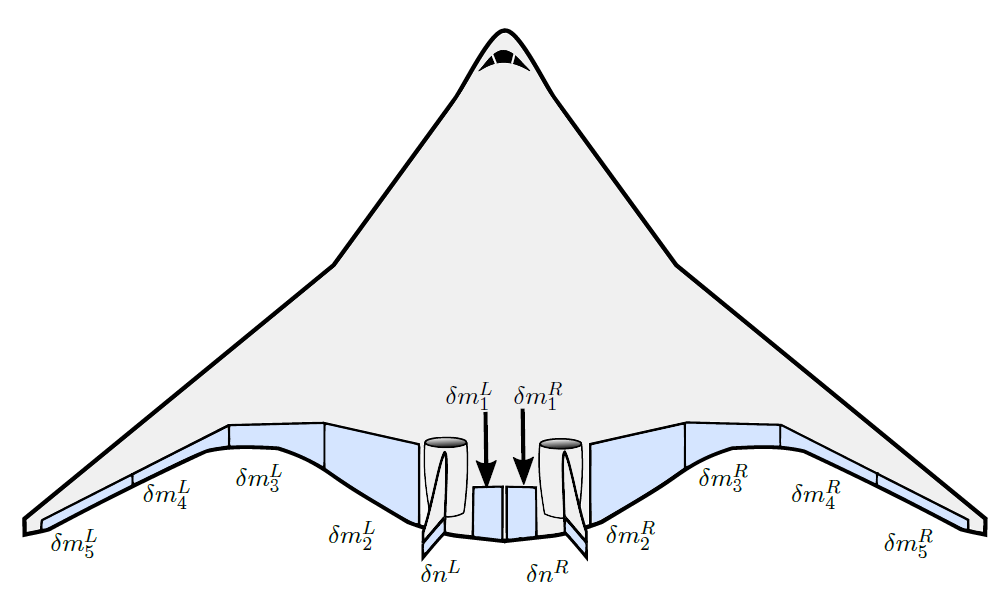
\includegraphics[scale=0.56]{Capitulo3/figs/2 12.png}
\caption{Airbus MAVERIC superficies de control \cite{Yann2016}}
\label{fig:  MAVERIC ACS}
\end{figure}
En \cite{Yann2016} se formulan y resuelven el problema del dimensionamiento de las superficies de control y el sistema de control de vuelo de una aeronave inestable BWB en lazo cerrado, usando herramientas matemáticas y numéricas de la comunidad de control. 
En resumen, se propusieron dos alternativas para el proceso iterativo:
\begin{enumerate}
    \item Diseño integrado del control y el ancho de banda de los actuadores.
    \item Diseño integrado del control y el dimensionamiento de las superficies de control aerodinámicas. 
\end{enumerate}
%
Las metodologías propuestas se aplicaron al problema de estabilidad longitudinal de MAVERIC BWB de Airbus aplicando diversas técnicas de control por asignación. 
En la Figura \ref{fig:  MAVERIC ACS} se observan las principales ACS de MAVERIC. Cuenta con diez ACS en el borde de fuga (cinco por semi-ala) y un par de timones de dirección en sus estabilizadores verticales que se localizan encima de su par de motores.

\section{Discusiones}

El concepto de aeronave de ala-integrada representa un avance significativo en el diseño aeronáutico al ofrecer ventajas notables en términos de eficiencia aerodinámica y economía de combustible.

El desarrollo histórico del concepto de BWB desde sus primeros diseños experimentales hasta los últimos modelos a escala propuestos por Boeing y Airbus muestran una trayectoria de innovación y mejora continua. Estudiar la evolución del BWB proporciona una perspectiva valiosa sobre las soluciones técnicas adoptadas y los desafíos superados por los ingenieros a lo largo del tiempo.

La construcción y prueba de modelos a escala desempeña un papel crucial en la validación y optimización de diseños de aeronaves. El análisis de los métodos y resultados de los modelos a escala proporciona información esencial sobre el comportamiento aerodinámico y estructural para aplicaciones futuras de mayor dimensión.

El diseño de sistemas de control de vuelo específicamente adaptados a aeronaves de ala-integrada es esencial para garantizar la estabilidad y maniobrabilidad. Resalta la técnica de control por asignación para el control de las aeronaves de ala-integrada. 

La comprensión detallada de los antecedentes presentados en este capítulo sienta las bases para el enfoque adoptado en el diseño y control de la aeronave de ala-integrada propuesta en esta tesis. Los conocimientos adquiridos a partir de estos antecedentes influyen en las decisiones de diseño y en la formulación de estrategias de control específicas para este proyecto.

Basado en la revisión de los antecedentes, se anticipa que el diseño y control de la aeronave de ala-integrada presentará desafíos de estabilidad y control que requerirán controladores robustos y que garanticen la estabilidad el lazo cerrado. 


%
%La formalización del problema integra el diseño y control en la interacción de parámetros físicos, como las ganancias de las leyes de control,  el tamaño del stick y el ancho de banda de los actuadores. Lo más destacable es la integración del diseño y control como un problema de optimización acotado con criterios de dimensionamiento formulados como restricciones en la norma de frecuencia. 

%La segunda contribución es un diseño mejorado respecto a las metodologías tradicionales, dado que con menos iteraciones se logró un mejor diseño óptimo. Esta aplicación clarifica el campo de aplicación para aplicar la metodología en la etapa de diseño preliminar. 

%Se logró la formulación del problema de ancho de banda de los actuadores bajo la forma de $H_2 / H_\infty$ del problema de optimización, con restricciones en la trasferencia del lazo cerrado para asegurar adecuadas operaciones. 
%Esta formulación permitió encontrar el mínimo del ancho de banda que garantizará un cierto nivel de rendimiento. 

%Una segunda aproximación incluyó el momento de fuerza de la superficie de control en el criterio de optimización. Se encontró que una solución óptima para el consumo energético de los actuadores era estabilizar la aeronave utilizando las superficies de control más pequeñas, sin embargo, menos de 2.5 hertz son suficientes para controlar la inestabilidad. 
%Los elevons deben ser dimensionados no sólo con respecto a criterios longitudinales sino laterales. 
%
%Para sobrepasar esta limitación, propusieron un estudio de optimización conjuntando todas las superficies de control, incluyendo longitudinales y laterales leyes de control, tomando en cuenta los requerimientos estructurales de las leyes de control. 
%Para este propósito se requirieron modelos computacionales parametrizados para poder dimensionar. 
%
%Se hizo una representación en espacio de estados discreta de alta precisión con CFD.
%
%, para después aproximar en base a este modelo en una representación continua LFR usando aproximación por mínimos cuadrados. 
%
%La parametrización de espacio de estados no se hizo para parámetros de vuelo variantes o inciertos, más bien para el tamaño físico de las superficies de control, buscando obtener un modelo adecuado para futuras optimizaciones de controladores con ganancias. 
%
%La parametrización del espacio de estados obtenida se optimiza bajo restricciones de rendimiento de lazo cerrado y restricciones de calidad de maniobra.
%
% utiliza un enfoque de dominio de frecuencia para establecer estas restricciones de calidad de manejo, escritas como amplitud máxima y tasa de control en respuesta a entradas exógenas o perturbaciones. 
%Mientras este enfoque ya se ha desarrollado en la literatura, se propone una discusión sobre el significado y las limitaciones de estos criterios en el dominio temporal, que debería ser útil para el ingeniero dispuesto a aplicar nuestras técnicas para el dimensionamiento de aeronaves. Escribir el problema de la síntesis de ganancias bajo la forma de un problema de satisfacción de una sola restricción también es un paso importante y facilita las rutinas de optimización que tienen en cuenta las estructuras prescritas para los controladores. 
%Finalmente, una vez escritas correctamente estas restricciones, se proponen tres procedimientos alternativos de optimización para resolver el problema de cálculo de ganancias y parámetros físicos, diferenciándose cada uno de los demás por las variables proporcionadas al optimizador.
%Una primera síntesis considera una optimización desacoplada y secuencial de la ley de control de vuelo, y el tramo de superficies de control después, aprovechando que el módulo de asignación de control está parametrizado por el tramo de superficies de control.
%Si bien mostramos que este enfoque conduce a un diseño sub-óptimo, aún encontramos interés presentándolo desde una perspectiva de aplicación industrial: de hecho, este enfoque no requiere una optimización de ganancias a través de la síntesis H1: los ingenieros pueden aplicar cualquier técnica de síntesis a la que estén acostumbrados y optimizar los parámetros físicos con ganancias fijas en un segundo paso. 
 %El diseño inicial de las superficies de control ahora resulta viable, con un margen uniforme en el tamaño de las superficies de control con respecto a los criterios de calidad de maniobra especificados. 
 %Mostramos que el intervalo exterior de las superficies de control se puede reducir en un 45 \% antes de que se saturen las restricciones. Curiosamente, la mayoría de los puntos de vuelo en la envolvente de vuelo resultan estar dimensionados por un criterio de balanceo; sin embargo, en la mayoría de los puntos de dimensionamiento, a bajo número de Mach y gran altitud, también se dimensionan por rechazo de turbulencia, lo que implícitamente significa que el control de inestabilidad dimensiona la aeronave.
 %
%Finalmente se muestra una seria dependencia del diseño optimizado y el método de asignación de control: Incluir el método la asignación dentro de la optimización lleva a mejorar el diseño sólo en cierto porcentaje. 
%
%Como conclusión, esta técnica dimensiona una aeronave directamente desde las especificaciones de lazo cerrado, en la dinámica longitudinal y lateral. Esta técnica es capaz de entregar información relevante en el dimensionamiento sobre la envolvente de vuelo, y dimensiona los criterios de las cualidades de maniobra. 
%Esta metodología puede ser muy útil para los diseñadores al momento de hacer decisiones en la siguiente generación de aeronaves. 
%
%Desde el punto de vista teórico el uso de rutinas de optimización eficientes para sintonizar los controladores ha abierto de nuevo un tema bien conocido en la comunidad de control: ¿son los requerimientos para una ley de control confiables? y si no, ¿cuál es su máximo nivel de operación? en efecto, algoritmos de optimización han probado ser muy eficientes en encontrar la mejor solución para un conjunto dado de restricciones. El trabajo del diseñador de control evolucionó de sintonizar las leyes de control hasta las especificaciones de la sintonización. 
%Herramientas de decisión que le indiquen al diseñador si las restricciones son realizables es un campo de investigación atractivo. 
%
%La arquitectura acoplada de BWB sería una vez más un reto y una oportunidad para la exploración combinada de todos los casos posibles de falla: Es un reto porque un corte (por ejemplo, un actuador atascado) implicaría un degrado de operación en todos los ejes, haciendo el análisis muy complejo comparado con las prácticas actuales, y una oportunidad porque la redundancia de las superficies de control crearía una nueva arquitectura mucho más resiliente para el caso de fallas. 











